\section{Input-to-state stability}
\label{sec:iss}

%\begin{itemize}
%\item ISS of a particle (use an appendix if long)
%\item Parameters need for a particle to be ISS
%\item Contrast with the empirical approach of Clerc and Kennedy??
%\item Use appendix for mean and variance analysis
%\end{itemize}

The properties of this system can be analyzed using the input-to-state stability of the position update component. 
Given an input-to-state stable position update component, we will see that the convergence of $ x_{i}(k) $ depends on bounds on $ x^{G}_{i}(k) $ and $ x^{P}_{i}(k) $.

Without loss of generality, we look at a one-dimension particle.
The parallel connection of input-to-state stable components reserves the input-to-state stability.

In our analysis of the PSO algorithm, we seek to understand how the particles converge to some position $ x^{*} $, which is intended (not guaranteed) by the algorithm to be the optimal position.
The convergence of this model means that $ v(k) \rightarrow 0 $ and $ x(k) \rightarrow x^{*} $.

\subsection{Input-to-state stability of the position update}

In this section, we briefly review the definition of input-to-state stability (ISS) including both the conditions that guarantee it and the bound that ISS implies\cite{Jiang2001857}. 
We then show that PSO satisfies this definition when the parameters of PSO are set in the requisite range.
We also derive the bounds implied by the ISS property.
We use the ISS property to find bounds on particle motion.

We first introduce several types of functions \cite{Jiang2001857}.
\begin{itemize}
\item $ K $-function $ \mathbb{K} $ : a function $ \alpha  : [ 0, a ) \rightarrow [ 0, \infty ) $ is continuous, strictly increasing and $ \alpha (0) = 0 $; it is a $ K_{\infty} $-function, if $ \alpha (s) \rightarrow \infty $ as $ s \rightarrow \infty $;
\item $ KL $-function $ \mathbb{KL} $ : a function $ \beta : [ 0, a ) \times [ 0 , \infty ) \rightarrow [ 0, \infty ) $ satisfies:
\begin{enumerate}
\item $ \forall t \geq 0 $, $ \beta (\cdot , t ) $ is a $ K $-function;
\item $ \forall s \geq 0 $, $ \beta (s, \cdot) $ is decreasing and $ \beta(s,t) \rightarrow 0 $ as $ t \rightarrow \infty $.
\end{enumerate}
%\item Positive-definite function: a function $ \gamma (s) > 0, \forall s > 0 $ and $ \gamma (0) = 0 $.
\item ISS-Lyapunov function $ V : \mathbb{R}^{n} \rightarrow \mathbb{R}_{\geq 0} $ satisfies:
\begin{enumerate}
\item $ \exists \alpha_{1}, \alpha_{2} \in \mathbb{K} $ such that 
$ \forall \xi \in \mathbb{R}^{n}, \alpha_{1} ( | \xi | ) \leq V( \xi ) \leq \alpha_{2}  ( | \xi | ) $.
\item $ \exists \alpha_{3} \in \mathbb{K}_{\infty} , \sigma \in \mathbb{K} $ such that $ \forall \xi \in \mathbb{R}^{n}, \forall \mu \in \mathbb{R}^{m}, V( f( \xi, \mu ) ) - V( \xi ) \leq - \alpha_{3} ( | \xi | ) + \sigma ( | \mu | ) $. 
\end{enumerate}
\end{itemize}

\begin{mydef}[Input-to-state stable]\cite{Jiang2001857}
\label{def:iss}
For a discrete-time system
\begin{equation}
\label{eq:dis_nonlinear}
x(k+1) = f( x(k) , u(k) ),
\end{equation}
with $ f(0,0) = 0 $
\footnote{This means that $ x = 0 $ is an equilibrium of the 0-input system.}, the system is \emph{(globally) input-to-state stable} if there exist a $ KL $-function $ \beta  $ and a $ K $-function $ \gamma $ such that, for each input $ u \in l^{m}_{\infty} $ and each $ \xi \in \mathbb{R}^{n} $, it holds that $  \forall k \in \mathbb{Z}^{+} $,
\begin{equation}
\label{eq:def_iss}
| x(k, \xi, u) | \leq \beta (| \xi |, k) + \gamma ( | u | ).
\end{equation}
\end{mydef}

The $ \beta () $ term in \eqref{eq:def_iss} defines an initial bound with a decaying property.
The $ \gamma () $ term in \eqref{eq:def_iss} defines a bound determined by the input.
This means that the influence $ \beta () $ term gradually decreases to zero and the position is bounded by a range determined by the bound on the input.
An ISS-Lyapunov function, defined above, can be used to prove the input-to-state stability of a system and analyze the state bound\cite{Jiang2001857}.
We will use the ISS-Lyapunov-function approach in the proof given later in this section.

\subsection{Conditions for input-to-state stability for position update in PSO}

Using the definition of the PSO position update as given in \eqref{eq:pso_up_linalg_simp}, PSO can be shown to be ISS as defined in definition \ref{def:iss}.

\begin{mythm}
\label{thm:iss}
The system \eqref{eq:pso_up_linalg_simp} is input-to-state stable, when $ | \lambda_{\max} ( A(k) ) | < 1 $.
%The system \eqref{eq:pso_up_linalg_simp} is input-to-state stable, if there exists a symmetric positive definite matrix $ P $ and a symmetric positive definite matrix $ Q' $ that has $ A(k)^{T} P A(k) - P = - Q(k) \leq - Q' $.
\begin{proof}

Let $ P $ be an identity matrix.
As $ | \lambda_{\max} ( A(k) ) | < 1 $, we have
$ \lVert A^{T}(k) P A(k) \rVert \leq \lVert P \rVert \lVert A(k) \rVert^{2} \leq \lVert P \rVert | \lambda_{\max} ( A(k) ) |^{2} < \lVert P \rVert $.
Because $ P $ is an identity matrix it is positive definite, and thus $ A^{T}(k) P A(k) $ is positive definite or positive semi-definite by definition.
So by positive definite ordering we have $ A^{T}(k) P A(k) < P $.

Let $ -Q(k) = A^{T}(k) P A(k) - P $. Since $ A^{T}(k) P A(k) < P $ then $ - Q(k) < 0 $ furthermore $ \exists Q' \forall k, Q(k) > Q' > 0 $. 

By the Lemma 3.5 in \cite{Jiang2001857}, if we can show that a proposed positive definite Lyapunov function is an ISS-Lyapunov function, then the system is ISS.

Define a Lyapunov function
\begin{equation}
\label{eq:lyapunov_v}
V( X(k) ) = X^{T} (k) P X(k).
\end{equation}
We can have
$
\lambda_{min}(P) | X(k) |^{2} \leq V( X(k) )\leq \lambda_{max}(P) | X(k) |^{2}
$ and $ \lambda_{min}(P) = \lambda_{max}(P) $.

Let $ \alpha_{1} ( \xi )= \lambda_{min} \xi^{2} $
and 
$ \alpha_{2} ( \xi )= \lambda_{max} \xi^{2} $,
we have $ V(x) $ satisfying condition 1 of the ISS-Lyapunov function definition.

By applying \eqref{eq:pso_up_linalg_simp} to $ V( X(k+1) ) - V( X(k) ) $, we have
\begin{equation}
\label{eq:lyapunov_delta2}
\begin{aligned}
& V( X(k+1) ) - V( X(k) ) \\
= & - X^{T}(k) [ A^{T}(k) P A(k) - P ] X(k)  \\
& + 2 X^{T}(k)  A^{T}(k) P B(k) U(k) + U^{T}(k) B^{T}(k) P B(k) U(k) \\
\leq & - X^{T}(k) Q' X(k) + 2 X^{T}(k)  A^{T}(k) P B(k) U(k) \\
& + U^{T}(k) B^{T}(k) P B(k) U(k) \\
\leq & - \lambda_{min}(Q') | X(k) |^{2} + 2  \lVert A^{T}(k) P B(k) \rVert | U(k) | | X(k) | \\
& + \lVert B^{T}(k) P B(k) \rVert | U(k) |^{2}.
\end{aligned}
\end{equation}

By completing the square, we have
\begin{equation}
\label{eq:lyapunov_delta4}
\begin{aligned}
& V( X(k+1) ) - V( X(k) ) \\
\leq & - \frac{1}{2} \lambda_{min}(Q') | X(k) |^{2} + [ \frac{2 \lVert A^{T}(k) P B(k) \rVert^{2}}{ ( \lambda_{min}(Q') )^{2} }  \\
& + \lVert B^{T}(k) P B(k) \rVert ] | U(k) |^{2}. 
\end{aligned}
\end{equation}

Because $ u^{P}(k) \in [0, 1] $, there exist an $ A' $ and $ B' $ such that $ \lVert A(k) \rVert \leq \lVert A' \rVert $ and $ \lVert B(k) \rVert \leq \lVert B' \rVert $.
We have $ \lVert A^{T}(k) P B(k) \rVert \leq \lVert A' \rVert \lVert P \rVert \lVert B' \rVert $ and $ \lVert B^{T}(k) P B(k) \rVert \leq \lVert P \rVert \lVert B' \rVert^{2} $.

Since the identity matrix $ P $ has $ || P || = 1 $:
\begin{equation}
\label{eq:lyapunov_delta5}
\begin{aligned}
& V( X(k+1) ) - V( X(k) ) \\
\leq & - \frac{1}{2} \lambda_{min}(Q') | X(k) |^{2} + [ \frac{2 \lVert A' \rVert^{2} \lVert B' \rVert^{2}}{ ( \lambda_{min}(Q') )^{2} } + \lVert B' \rVert^{2} ] | U(k) |^{2}.
\end{aligned}
\end{equation}

Let
$ \alpha_{3} ( \xi )= \frac{1}{2} \lambda_{min}(Q') \xi^{2} $,
and
$ \sigma ( \xi ) = [ \frac{2 \lVert A' \rVert^{2} \lVert B' \rVert^{2}}{ ( \lambda_{min}(Q') )^{2} } +  \lVert B' \rVert^{2} ] \xi^{2} $.
Thus we have $  V( X(k+1) ) - V( X(k) ) $ satisfying condition 2 of the ISS-Lyapunov function definition and
so \eqref{eq:lyapunov_v} is an ISS-Lyapunov function.
Using Lemma 3.5 in \cite{Jiang2001857}, the position update component of PSO \eqref{eq:pso_up_linalg_simp} is input-to-state stable.

\end{proof}
\end{mythm}

Note that in using \eqref{eq:pso_up_linalg_simp} with $ x^{R} = x^{*} $,
$ [ v(k), x(k) - x^{*} ]^{T} = [0, 0]^{T} $ is an equilibrium position when the input $ [ x^{G}(k) - x^{*} , x^{P}(k) - x^{*} ]^{T} = [0, 0]^{T} $.
For an arbitrary optimization problem $ x^{R} $ would typically not be at the origin. 
In such a problem, input-to-state stability means that the boundaries of $ | v(k) | $ and $ | x(k) - x^{R} | $ would be transformed and thus determined by $ | x^{G}(k) - x^{R} | $ and $ | x^{P}(k) - x^{R} | $,
but the properties of ISS still apply independent of where the function is centered.
Having proven that PSO is ISS we can now state a bound on particle position.

\begin{mythm}
\label{thm:state_bound}
Given the bound on the input $ \lVert u \rVert $ in the position update component, we have the bound on the particle position from \eqref{eq:pso_up_linalg_simp}.
\begin{equation}
\label{eq:state_bound}
\forall k, 
| x(k+1) - x^{R} | \leq \max ( | x(0) - x^{R} | , \gamma ( | [ x^{G}(k) - x^{R}, x^{P}(k) - x^{R} ]^{T} | ) ),
\end{equation}
in which $ \gamma = \alpha_{3}^{-1} \circ \sigma $.

The $ \max $ part is needed to account for the effect of the starting point, represented by the first parameter. Eventually the effect of the starting point no longer affects the system, formally:
\begin{equation}
\label{eq:state_bound:conv}
\exists T, \forall k \geq T, 
|  x(k+1) - x^{R} | \leq \gamma ( | [ x^{G}(k) - x^{R}, x^{P}(k) - x^{R} ]^{T} | ).
\end{equation}
\begin{proof}
As we have the update equation as
$ X(k+1) = A(k) X(k) + B(k) U(k) $, we can derive 
\begin{equation}
X(k+1) = ( \prod_{k}^{i=0} A(i) ) X(0) + \sum_{i=0}^{k} [ ( \prod_{j=0}^{i-1} A(j) ) B(i) U(i)  ] 
\end{equation}
by recursively applying it.

By the property of matrix norm, we have
\begin{equation}
| X(k+1) | \leq ( \prod_{i=0}^{k} \lVert A(i) \rVert ) | X(0) | + \sum_{i=0}^{k} [ ( \prod_{j=0}^{i-1} \lVert A(j) \rVert ) \lVert B(i) \rVert | U(i) |  ].
\end{equation}

$ \forall i \in [0, k] $, let $ \lVert A(i) \rVert \leq \lVert A \rVert $, $  \lVert B(i) \rVert \leq \lVert B \rVert $ and $ | U(k) | = [ x^{G}(k) - x^{R}, x^{P}(k) - x^{R} ]^{T} $, we have
\begin{equation}
\label{eq:bound:final}
\begin{aligned}
& |  x(k+1) - x^{R} | \leq | X(k+1) | \\
& \leq ( \lVert A \rVert )^{k+1} | X(0) | + \sum_{i=0}^{k} [ ( \lVert A \rVert )^{i} \lVert B \rVert | U(i) |  ] \\
& = ( \lVert A \rVert )^{k+1} | X(0) | + \frac{1 - ( \lVert A \rVert )^{k+1} }{1 - \lVert A \rVert }  \lVert B \rVert | U(i) |
\end{aligned}
\end{equation}

%The boundary will be a function of $ bound ( \lVert A \rVert, \lVert B \rVert, | X(0) |, | U |, k ) $.
%Thus the minimum boundary is $ \min_{k} bound ( \lVert A \rVert, \lVert B \rVert, | X(0) |, | U |, k ) $.
%When we have $ \lVert A \rVert < 1 $, 
%$ ( \lVert A \rVert )^{k+1} \rightarrow 0 $ and
%$ \frac{1 - (\lVert A \rVert )^{k+1} }{1 - \lVert A \rVert} \rightarrow \frac{1}{1 - \lVert A \rVert } $
%as $ k \rightarrow \infty $.

$ ( \lVert A \rVert )^{k+1} $ shows the decay term and $ \frac{1 - ( \lVert A \rVert )^{k+1} }{1 - \lVert A \rVert }  \lVert B \rVert $ makes the boundary function $ \gamma () $.

\end{proof}
\end{mythm}

Figure \ref{fig:boundary} gives an example on how a particle's boundary is determined by the personal best and global best.

\begin{figure}
\centering
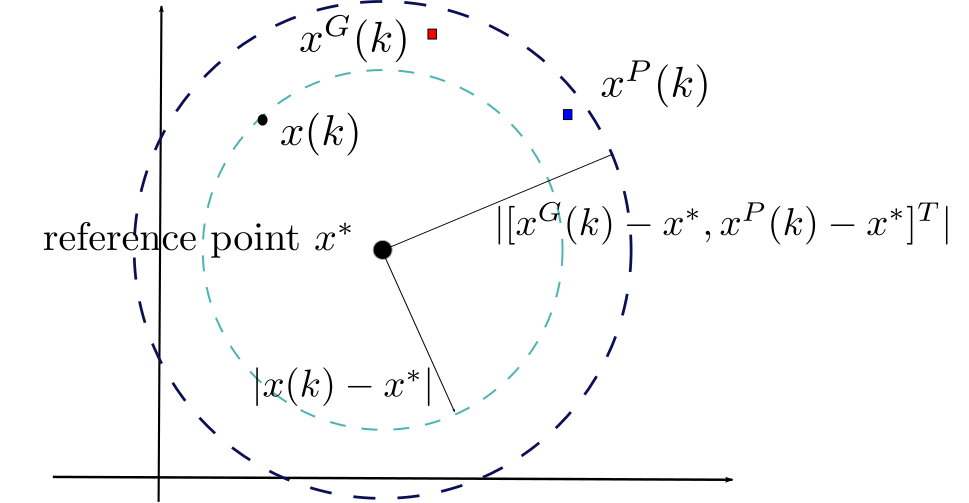
\includegraphics[width=0.6\linewidth]{./fig/boundary}
\caption{A bound on a particle's position by a reference point $ x^{*} $ from Equation \ref{eq:state_bound:conv}.
The ratio of wo radii indicates $ \gamma $.}
\label{fig:boundary}
\end{figure}

\begin{mycoro}
\label{coro:param_unit_disc}
Write $ A(k) = 
\begin{bmatrix}
\chi & - \chi \phi \\
\chi & 1 - \chi \phi
\end{bmatrix}
$, in which
$ \phi \in [0,  \phi^{P} + \phi^{G} ] $ and $ \chi \in ( 0, 1 ) $.
When $ \phi \in (0 , \frac{2(1+\chi)}{\chi} ) $, the system \eqref{eq:pso_up_linalg_simp} is input-to-state stable.
\begin{proof}
Let $ a = (1 + \chi) - \chi \phi $. 
The eigenvalues of $ A(k) $ are
$ \lambda = \frac{ a \pm \sqrt{ a^{2} - 4 \chi } }{2} $.

\begin{enumerate}
\item If $ a^{2} \geq 4 \chi $, we have $ a \geq 2 \sqrt{\chi} $ or $ a \leq - 2 \sqrt{\chi} $.

If $ a \geq 2 \sqrt{\chi} $, then $ | \lambda_{\max} | < 1 $ derives $ 0 < \frac{a-\sqrt{a^{2}-4\chi}}{2} \leq \frac{a+\sqrt{a^{2}-4\chi}}{2} < 1 $.
It means that $ 2 \sqrt{ \chi } \leq a < 1 + \chi $.

If $ a \leq 2 \sqrt{\chi} $, then $ | \lambda_{\max} | < 1 $ derives $ -1 < \frac{a-\sqrt{a^{2}-4\chi}}{2} \leq \frac{a+\sqrt{a^{2}-4\chi}}{2} < 0 $.
It means that $ - (\chi+1) < a \leq - 2 \sqrt{\chi} $.

\item If $ a^{2} \geq 4 \chi $, we have $ - 2 \sqrt{\chi} < a < 2 \sqrt{\chi} $.

$ | \lambda_{\max} | < 1 $ derives $ \frac{ a^{2} }{4} + \frac{ a^{2} - 4\chi }{4} < 1 $.
It means that $ - 2 \sqrt{ 2(1+\chi) } < a < 2 \sqrt{ 2(1+\chi) } $.
Because $ \sqrt{ 2(1+\chi) } > 2 \sqrt{ \chi } $, we have $ - 2 \sqrt{\chi} < a < 2 \sqrt{\chi} $.
\end{enumerate}
Combining these two cases, we have  $ - (1 + \chi) < a < 1 + \chi $.
It equals to $ \phi \in (0 , \frac{2(1+\chi)}{\chi} ) $.

\end{proof}
\end{mycoro}

Figure \ref{fig:paramSpace} shows the parameter space.
The x-axis is $ \phi = \phi^{P} + \phi^{G} $ and the y-axis is $ \chi $.
The stable region in red is obtained from eigenvalue test on Theorem \ref{thm:iss} and the yellow boundary is obtained from Corollary \ref{coro:param_unit_disc}.
\begin{figure}
\centering
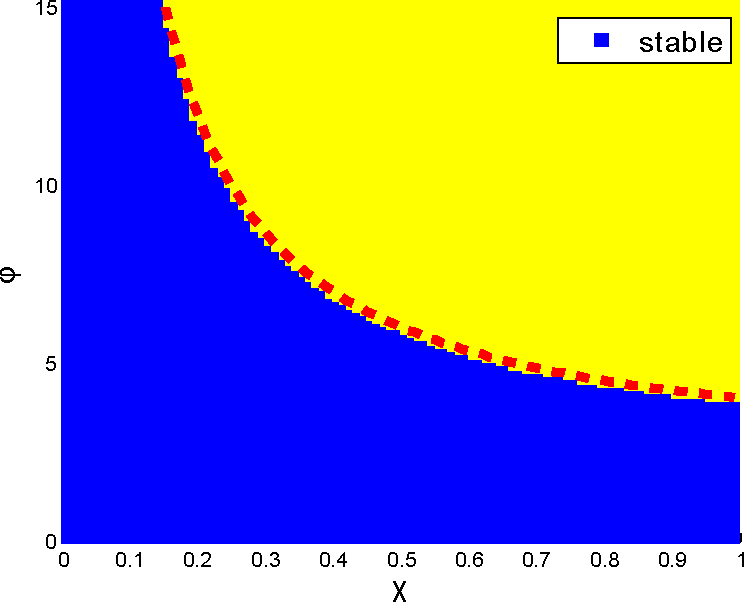
\includegraphics[width=0.5\linewidth]{./fig/param2}
\caption{Parameter space}
\label{fig:paramSpace}
\end{figure}


%Since by Theorem \ref{thm:iss} PSO is ISS, and therefore by Corollary \ref{coro:state_bound} the stability of the cascade system depends on the output of the input update component. We can say:
%\begin{enumerate}
%\item If the input update component generates converging personal best and global best, the bound of the particle position will converge;
%\item If the personal best and global best vary within a bound, the particle will converge within a bound;
%\item If the personal best and global best become constant, the particle will converge to a point.
%\end{enumerate}
%Furthermore, by equation \eqref{eq:state_bound}, we know that the convergence of a particle's position $ x(k) $ to $ x^{*} $ depends on how $ x^{P}(k) $ and $ x^{G}(k) $ converge to $ x^{*} $, if the position update component is input-to-state stable.
%In particular, the boundary of the distance between a particle's position and  $ x^{*} $ is determined by the initial distance $ x(0) -  x^{*} $, $ x^{P}(k) -  x^{*} $ and $ x^{G}(k) -  x^{*} $.

%Answer two questions here
% a) why we need iss of position update 
% b) what else do we need for iss

The input-to-state stability of the position update component makes the movement of a particle bounded in a range that covers the global best and the personal best.
This property provides the chance that the particle exploits the regions near around the personal best and the global best.
We can have:
\begin{enumerate}
\item If the personal best and global best converge, the bound of the particle position will converge;
\item If the personal best and global best vary within a bound, the particle will converge within a bound;
\item If the personal best and global best become constant, the particle will converge to a point.
\end{enumerate}
Furthermore, by \eqref{eq:state_bound}, we know that the convergence of a particle's position $ x(k) $ to $ x^{R} $ depends on how $ x^{P}(k) $ and $ x^{G}(k) $ converge to $ x^{R} $, if the position update component is input-to-state stable.
In particular, the boundary of the distance between a particle's position and  $ x^{R} $ is determined by the initial distance $ x(0) -  x^{R} $, $ x^{P}(k) -  x^{R} $ and $ x^{G}(k) -  x^{R} $.
Conversely, if the position update component is not input-to-state stable, the movement of the particle will diverge from the global best and the personal best.
The design of the exploitation by the personal best and the global best is lost.
%As in Figure \ref{fig:sys_flow}, the position update component and the input update component are serially connected.
When the position update component is input-to-state stable, the input-to-state stability of the particle is determined by the input-to-state stability of the personal best update component.
However, the input-to-state stability of the input update component depends on the fitness distribution, which could not be guaranteed in many cases.
In section \ref{sec:particle}, we will analyze the behavior of the particle when the position update component is input-to-state stable.
We will later extend the analysis to the swarm in section \ref{sec:swarm}.



